% !TeX TXS-program:compile = txs:///knit2pdf
\documentclass[12pt]{mwart}\usepackage[]{graphicx}\usepackage[]{color}
% maxwidth is the original width if it is less than linewidth
% otherwise use linewidth (to make sure the graphics do not exceed the margin)
\makeatletter
\def\maxwidth{ %
  \ifdim\Gin@nat@width>\linewidth
    \linewidth
  \else
    \Gin@nat@width
  \fi
}
\makeatother

\definecolor{fgcolor}{rgb}{0.345, 0.345, 0.345}
\newcommand{\hlnum}[1]{\textcolor[rgb]{0.686,0.059,0.569}{#1}}%
\newcommand{\hlstr}[1]{\textcolor[rgb]{0.192,0.494,0.8}{#1}}%
\newcommand{\hlcom}[1]{\textcolor[rgb]{0.678,0.584,0.686}{\textit{#1}}}%
\newcommand{\hlopt}[1]{\textcolor[rgb]{0,0,0}{#1}}%
\newcommand{\hlstd}[1]{\textcolor[rgb]{0.345,0.345,0.345}{#1}}%
\newcommand{\hlkwa}[1]{\textcolor[rgb]{0.161,0.373,0.58}{\textbf{#1}}}%
\newcommand{\hlkwb}[1]{\textcolor[rgb]{0.69,0.353,0.396}{#1}}%
\newcommand{\hlkwc}[1]{\textcolor[rgb]{0.333,0.667,0.333}{#1}}%
\newcommand{\hlkwd}[1]{\textcolor[rgb]{0.737,0.353,0.396}{\textbf{#1}}}%
\let\hlipl\hlkwb

\usepackage{framed}
\makeatletter
\newenvironment{kframe}{%
 \def\at@end@of@kframe{}%
 \ifinner\ifhmode%
  \def\at@end@of@kframe{\end{minipage}}%
  \begin{minipage}{\columnwidth}%
 \fi\fi%
 \def\FrameCommand##1{\hskip\@totalleftmargin \hskip-\fboxsep
 \colorbox{shadecolor}{##1}\hskip-\fboxsep
     % There is no \\@totalrightmargin, so:
     \hskip-\linewidth \hskip-\@totalleftmargin \hskip\columnwidth}%
 \MakeFramed {\advance\hsize-\width
   \@totalleftmargin\z@ \linewidth\hsize
   \@setminipage}}%
 {\par\unskip\endMakeFramed%
 \at@end@of@kframe}
\makeatother

\definecolor{shadecolor}{rgb}{.97, .97, .97}
\definecolor{messagecolor}{rgb}{0, 0, 0}
\definecolor{warningcolor}{rgb}{1, 0, 1}
\definecolor{errorcolor}{rgb}{1, 0, 0}
\newenvironment{knitrout}{}{} % an empty environment to be redefined in TeX

\usepackage{alltt}
\usepackage[utf8]{inputenc}
\usepackage[T1,plmath]{polski}
\usepackage{lmodern}

\usepackage{amssymb}
\usepackage{graphicx}
\usepackage{amsmath}
\usepackage{amsthm}
\usepackage[hidelinks]{hyperref}
\usepackage{float}

\title{Sprawozdanie 1}
\author{Aleksander Jakóbczyk i Kacper Pasterniak}
\date{}
\IfFileExists{upquote.sty}{\usepackage{upquote}}{}
\begin{document}
	\maketitle 
	

	
	\section*{Lista 1}
  \subsection*{Zad 1}
  Sporządzić tablice liczności dla zmiennych \textit{Temperature} oraz \textit{Preference} biorąc pod uwagę wszystkie dane, jak również w podgrupach ze względu na zmienną \textit{Water Softness}:
  \subsubsection*{Detergent}
\begin{knitrout}\small
\definecolor{shadecolor}{rgb}{0.969, 0.969, 0.969}\color{fgcolor}\begin{kframe}
\begin{alltt}
\hlstd{Detergent.df} \hlkwb{<-} \hlkwd{data.frame}\hlstd{(Detergent)}
\hlstd{Detergent.df} \hlopt \hlkwd{group_by}\hlstd{(Temperature)} \hlopt \hlkwd{summarise}\hlstd{(}\hlkwc{n} \hlstd{=} \hlkwd{sum}\hlstd{(Freq))}
\end{alltt}
\begin{verbatim}
## # A tibble: 2 x 2
##   Temperature     n
##   <fct>       <dbl>
## 1 High          369
## 2 Low           639
\end{verbatim}
\begin{alltt}
\hlstd{Detergent.df} \hlopt \hlkwd{filter}\hlstd{(Water_softness} \hlopt{==} \hlstr{"Soft"}\hlstd{)} \hlopt
  \hlkwd{group_by}\hlstd{(Temperature)} \hlopt \hlkwd{summarise}\hlstd{(}\hlkwc{n} \hlstd{=} \hlkwd{sum}\hlstd{(Freq))}
\end{alltt}
\begin{verbatim}
## # A tibble: 2 x 2
##   Temperature     n
##   <fct>       <dbl>
## 1 High          104
## 2 Low           222
\end{verbatim}
\begin{alltt}
\hlstd{Detergent.df} \hlopt \hlkwd{filter}\hlstd{(Water_softness} \hlopt{==} \hlstr{"Medium"}\hlstd{)} \hlopt
  \hlkwd{group_by}\hlstd{(Temperature)} \hlopt \hlkwd{summarise}\hlstd{(}\hlkwc{n} \hlstd{=} \hlkwd{sum}\hlstd{(Freq))}
\end{alltt}
\begin{verbatim}
## # A tibble: 2 x 2
##   Temperature     n
##   <fct>       <dbl>
## 1 High          126
## 2 Low           218
\end{verbatim}
\begin{alltt}
\hlstd{Detergent.df} \hlopt \hlkwd{filter}\hlstd{(Water_softness} \hlopt{==} \hlstr{"Hard"}\hlstd{)} \hlopt
  \hlkwd{group_by}\hlstd{(Temperature)} \hlopt \hlkwd{summarise}\hlstd{(}\hlkwc{n} \hlstd{=} \hlkwd{sum}\hlstd{(Freq))}
\end{alltt}
\begin{verbatim}
## # A tibble: 2 x 2
##   Temperature     n
##   <fct>       <dbl>
## 1 High          139
## 2 Low           199
\end{verbatim}
\end{kframe}
\end{knitrout}

  \subsubsection*{Preference}

\begin{knitrout}\small
\definecolor{shadecolor}{rgb}{0.969, 0.969, 0.969}\color{fgcolor}\begin{kframe}
\begin{alltt}
\hlcom{# Detergent.df %>% group_by(Preference) %>% summarise(n = sum(Freq))}
\hlstd{Detergent.df} \hlopt \hlkwd{filter}\hlstd{(Water_softness} \hlopt{==} \hlstr{"Soft"}\hlstd{)} \hlopt
  \hlkwd{group_by}\hlstd{(Preference)} \hlopt \hlkwd{summarise}\hlstd{(}\hlkwc{n} \hlstd{=} \hlkwd{sum}\hlstd{(Freq))}
\end{alltt}
\begin{verbatim}
## # A tibble: 2 x 2
##   Preference     n
##   <fct>      <dbl>
## 1 Brand X      168
## 2 Brand M      158
\end{verbatim}
\begin{alltt}
\hlstd{Detergent.df} \hlopt \hlkwd{filter}\hlstd{(Water_softness} \hlopt{==} \hlstr{"Medium"}\hlstd{)} \hlopt
  \hlkwd{group_by}\hlstd{(Preference)} \hlopt \hlkwd{summarise}\hlstd{(}\hlkwc{n} \hlstd{=} \hlkwd{sum}\hlstd{(Freq))}
\end{alltt}
\begin{verbatim}
## # A tibble: 2 x 2
##   Preference     n
##   <fct>      <dbl>
## 1 Brand X      169
## 2 Brand M      175
\end{verbatim}
\begin{alltt}
\hlstd{Detergent.df} \hlopt \hlkwd{filter}\hlstd{(Water_softness} \hlopt{==} \hlstr{"Hard"}\hlstd{)} \hlopt
  \hlkwd{group_by}\hlstd{(Preference)} \hlopt \hlkwd{summarise}\hlstd{(}\hlkwc{n} \hlstd{=} \hlkwd{sum}\hlstd{(Freq))}
\end{alltt}
\begin{verbatim}
## # A tibble: 2 x 2
##   Preference     n
##   <fct>      <dbl>
## 1 Brand X      171
## 2 Brand M      167
\end{verbatim}
\end{kframe}
\end{knitrout}
\begin{kframe}
\begin{alltt}
\hlstd{data} \hlkwb{<-} \hlkwd{matrix}\hlstd{(}\hlkwd{c} \hlstd{(}\hlnum{32}\hlstd{,}\hlnum{44}\hlstd{,}
                  \hlnum{22}\hlstd{,}\hlnum{38}\hlstd{),} \hlnum{2}\hlstd{,} \hlnum{2}\hlstd{,} \hlkwc{byrow} \hlstd{= T)}


\hlkwd{print}\hlstd{(data)}
\end{alltt}
\end{kframe}     [,1] [,2]
[1,]   32   44
[2,]   22   38


  \subsection*{Zad 2}
  Sporządzić tabelę wielodzielczą uwzględniającą zmienną \textit{Temperature} i \textit{Water Softness}:
\begin{knitrout}
\definecolor{shadecolor}{rgb}{0.969, 0.969, 0.969}\color{fgcolor}\begin{kframe}
\begin{alltt}
\hlkwd{ftable}\hlstd{(Detergent,} \hlkwc{col.vars} \hlstd{=} \hlstr{"Temperature"}\hlstd{,} \hlkwc{row.vars} \hlstd{=} \hlstr{"Water_softness"}\hlstd{)}
\end{alltt}
\begin{verbatim}
##                Temperature High Low
## Water_softness                     
## Soft                        104 222
## Medium                      126 218
## Hard                        139 199
\end{verbatim}
\begin{alltt}
\hlkwd{structable}\hlstd{(Temperature} \hlopt{~} \hlstd{Water_softness, Detergent)} \hlopt \hlkwd{addmargins}\hlstd{()}
\end{alltt}
\begin{verbatim}
##               Temperature
## Water_softness High Low  Sum
##         Soft    104 222  326
##         Medium  126 218  344
##         Hard    139 199  338
##         Sum     369 639 1008
\end{verbatim}
\end{kframe}
\end{knitrout}

\subsection*{Zad 3}
Sporządzić wykres kołowy i słupkowy dla zmiennej \textit{Water Softness}:
\begin{knitrout}
\definecolor{shadecolor}{rgb}{0.969, 0.969, 0.969}\color{fgcolor}\begin{kframe}
\begin{alltt}
\hlkwd{par}\hlstd{(}\hlkwc{mar} \hlstd{=} \hlkwd{c}\hlstd{(}\hlnum{2}\hlstd{,} \hlnum{2}\hlstd{,} \hlnum{0.5}\hlstd{,} \hlnum{1}\hlstd{))}
\hlstd{A} \hlkwb{<-} \hlkwd{apply}\hlstd{(Detergent,} \hlstr{"Water_softness"}\hlstd{, sum)}
\hlkwd{barplot}\hlstd{(A,}\hlkwc{ylim}\hlstd{=}\hlkwd{c}\hlstd{(}\hlnum{0}\hlstd{,}\hlnum{350}\hlstd{))}
\end{alltt}
\end{kframe}\begin{figure}[H]
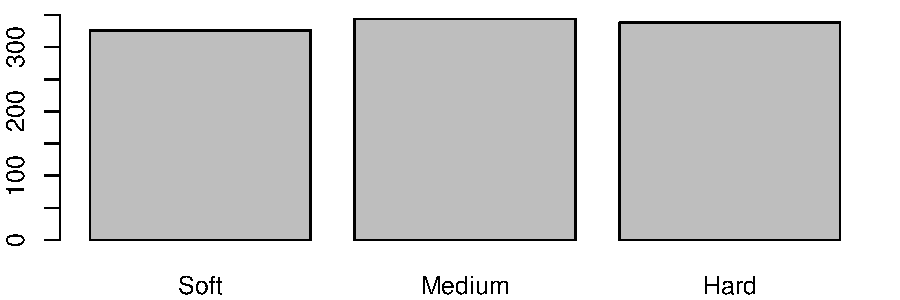
\includegraphics[width=\maxwidth]{figure/fig_1-1} \caption{\label{fig:1}Wykres słupkowy dla zmiennej \text{\textit{Water Softness}}.}\label{fig:fig_1}
\end{figure}

\end{knitrout}
\begin{knitrout}
\definecolor{shadecolor}{rgb}{0.969, 0.969, 0.969}\color{fgcolor}\begin{kframe}
\begin{alltt}
\hlkwd{par}\hlstd{(}\hlkwc{mar} \hlstd{=} \hlkwd{c}\hlstd{(}\hlnum{0}\hlstd{,}\hlnum{0}\hlstd{,}\hlnum{0}\hlstd{,}\hlnum{0}\hlstd{))}
\hlkwd{pie}\hlstd{(A)}
\end{alltt}
\end{kframe}\begin{figure}[H]
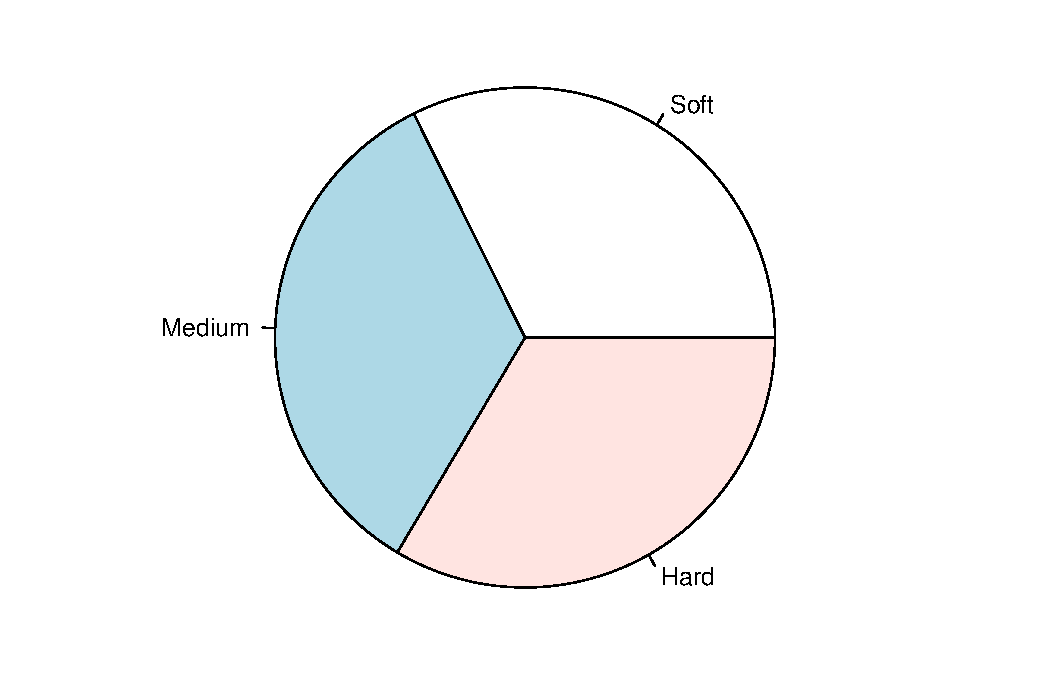
\includegraphics[width=\maxwidth]{figure/fig_2-1} \caption{\label{fig:2}Wykresy kołowy dla zmiennej \text{\textit{Water Softness}}.}\label{fig:fig_2}
\end{figure}

\end{knitrout}
  \subsection*{Zad 4}
  Sporządzić wykresy mozaikowe odpowiadające rozpatrywanym danym.
\begin{knitrout}
\definecolor{shadecolor}{rgb}{0.969, 0.969, 0.969}\color{fgcolor}\begin{kframe}
\begin{alltt}
\hlkwd{par}\hlstd{(}\hlkwc{mar} \hlstd{=} \hlkwd{c}\hlstd{(}\hlnum{2}\hlstd{,} \hlnum{2}\hlstd{,} \hlnum{2}\hlstd{,} \hlnum{2}\hlstd{))}
\hlkwd{mosaicplot}\hlstd{(}\hlopt{~}\hlstd{Water_softness}\hlopt{+}\hlstd{Preference,} \hlkwc{data} \hlstd{= Detergent)}
\end{alltt}
\end{kframe}\begin{figure}[H]
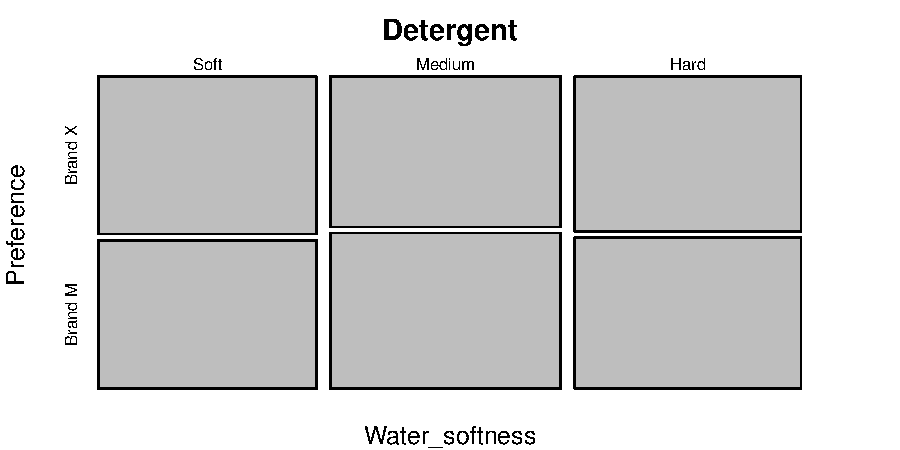
\includegraphics[width=\maxwidth]{figure/fig_3-1} \caption{\label{fig:3}Wykres mozaikowy dla \text{\textit{Preference}} i \text{\textit{Water softness}}}\label{fig:fig_3}
\end{figure}

\end{knitrout}
\begin{knitrout}
\definecolor{shadecolor}{rgb}{0.969, 0.969, 0.969}\color{fgcolor}\begin{kframe}
\begin{alltt}
\hlkwd{par}\hlstd{(}\hlkwc{mar} \hlstd{=} \hlkwd{c}\hlstd{(}\hlnum{2}\hlstd{,} \hlnum{2}\hlstd{,} \hlnum{2}\hlstd{,} \hlnum{2}\hlstd{))}
\hlkwd{mosaicplot}\hlstd{(}\hlopt{~}\hlstd{M_User}\hlopt{+}\hlstd{Preference,} \hlkwc{data} \hlstd{= Detergent)}
\end{alltt}
\end{kframe}\begin{figure}[H]
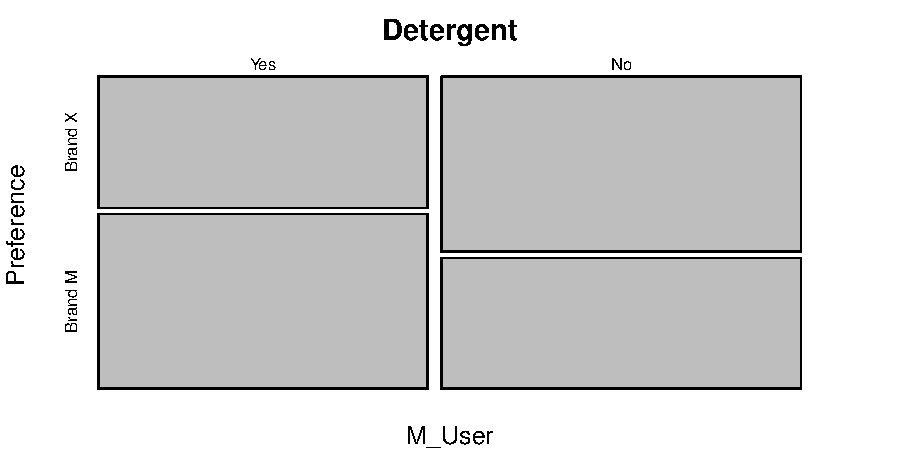
\includegraphics[width=\maxwidth]{figure/fig_4-1} \caption{\label{fig:4}Wykres mozaikowy dla \text{\textit{Preference}} i \text{\textit{M User}}.}\label{fig:fig_4}
\end{figure}

\end{knitrout}
\begin{knitrout}
\definecolor{shadecolor}{rgb}{0.969, 0.969, 0.969}\color{fgcolor}\begin{kframe}
\begin{alltt}
\hlkwd{par}\hlstd{(}\hlkwc{mar} \hlstd{=} \hlkwd{c}\hlstd{(}\hlnum{2}\hlstd{,} \hlnum{2}\hlstd{,} \hlnum{2}\hlstd{,} \hlnum{2}\hlstd{))}
\hlkwd{mosaicplot}\hlstd{(}\hlopt{~}\hlstd{Temperature}\hlopt{+}\hlstd{Preference,} \hlkwc{data} \hlstd{= Detergent)}
\end{alltt}
\end{kframe}\begin{figure}[H]
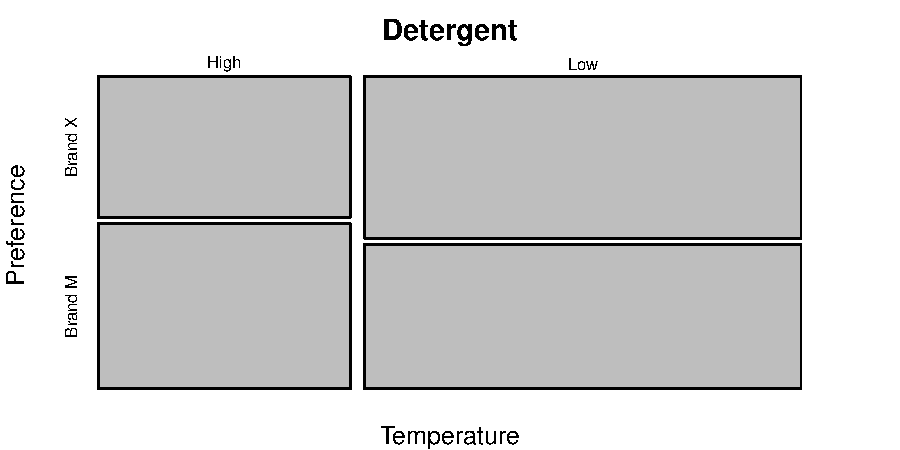
\includegraphics[width=\maxwidth]{figure/fig_5-1} \caption{\label{fig:5}Wykres mozaikowy dla \text{\textit{Preference}} i \text{\textit{Temperature}}.}\label{fig:fig_5}
\end{figure}

\end{knitrout}
Wykresy mozaikowe są bardzo proste w analizie. Wykres tworzy nam prostokąty, dzięki czemu łatwo zauważyć które kombinacje zmiennych są najliczniejsze. Wysokość takiego prostokąta odpowiada liczności zmiennej na osi OX, a szerokość odpowiada liczności zmiennej na osi OY.
\section*{Lista 2}
\subsection*{Zad 1}
Zapoznać się z funkcją \textit{sample} (w pakiecie \textit{stats}). Napisać fragment programu, którego celem jest wylosowanie próbki rozmiaru około 1/10 liczby przypadków danej
bazy danych (pewnej hipotetycznej), ze zwracaniem oraz bez zwracania.
\newline\newline
Będziemy korzystać z funkcji $sample$. Wylosujemy elementy z bazy danych o nazwie $mtcars$. Jest to zbiór informacji na temat specyfikacji różnych samochodów, poniżej widzimy pięć pierwszych wierszy:
\begin{knitrout}
\definecolor{shadecolor}{rgb}{0.969, 0.969, 0.969}\color{fgcolor}\begin{kframe}
\begin{alltt}
\hlkwd{head}\hlstd{(mtcars,}\hlnum{5}\hlstd{)}
\end{alltt}
\begin{verbatim}
##                    mpg cyl disp  hp drat    wt  qsec vs am gear carb
## Mazda RX4         21.0   6  160 110 3.90 2.620 16.46  0  1    4    4
## Mazda RX4 Wag     21.0   6  160 110 3.90 2.875 17.02  0  1    4    4
## Datsun 710        22.8   4  108  93 3.85 2.320 18.61  1  1    4    1
## Hornet 4 Drive    21.4   6  258 110 3.08 3.215 19.44  1  0    3    1
## Hornet Sportabout 18.7   8  360 175 3.15 3.440 17.02  0  0    3    2
\end{verbatim}
\end{kframe}
\end{knitrout}

\subsubsection*{Losowanie ze zwracaniem:} 
\begin{knitrout}
\definecolor{shadecolor}{rgb}{0.969, 0.969, 0.969}\color{fgcolor}\begin{kframe}
\begin{alltt}
\hlstd{ind} \hlkwb{<-} \hlkwd{sample}\hlstd{(}\hlkwc{x}\hlstd{=}\hlkwd{nrow}\hlstd{(mtcars),}\hlkwc{size}\hlstd{=}\hlkwd{nrow}\hlstd{(mtcars)}\hlopt{/}\hlnum{10}\hlstd{,}\hlkwc{replace}\hlstd{=}\hlnum{TRUE}\hlstd{)}
\end{alltt}
\end{kframe}
\end{knitrout}
Wylosowane indeksy:
\begin{knitrout}
\definecolor{shadecolor}{rgb}{0.969, 0.969, 0.969}\color{fgcolor}\begin{kframe}
\begin{alltt}
\hlstd{ind}
\end{alltt}
\begin{verbatim}
## [1]  5  9 29
\end{verbatim}
\end{kframe}
\end{knitrout}
Wylosowane elementy z bazy danych:
\begin{knitrout}\small
\definecolor{shadecolor}{rgb}{0.969, 0.969, 0.969}\color{fgcolor}\begin{kframe}
\begin{alltt}
\hlstd{mtcars[ind,]}
\end{alltt}
\begin{verbatim}
##                    mpg cyl  disp  hp drat   wt  qsec vs am gear carb
## Hornet Sportabout 18.7   8 360.0 175 3.15 3.44 17.02  0  0    3    2
## Merc 230          22.8   4 140.8  95 3.92 3.15 22.90  1  0    4    2
## Ford Pantera L    15.8   8 351.0 264 4.22 3.17 14.50  0  1    5    4
\end{verbatim}
\end{kframe}
\end{knitrout}
\textbf{Losowanie bez zwracania:} 
\begin{knitrout}
\definecolor{shadecolor}{rgb}{0.969, 0.969, 0.969}\color{fgcolor}\begin{kframe}
\begin{alltt}
\hlstd{ind} \hlkwb{<-} \hlkwd{sample}\hlstd{(}\hlkwc{x}\hlstd{=}\hlkwd{nrow}\hlstd{(mtcars),}\hlkwc{size}\hlstd{=}\hlkwd{nrow}\hlstd{(mtcars)}\hlopt{/}\hlnum{10}\hlstd{,}\hlkwc{replace}\hlstd{=}\hlnum{FALSE}\hlstd{)}
\end{alltt}
\end{kframe}
\end{knitrout}
Wylosowane indeksy:
\begin{knitrout}
\definecolor{shadecolor}{rgb}{0.969, 0.969, 0.969}\color{fgcolor}\begin{kframe}
\begin{alltt}
\hlstd{ind}
\end{alltt}
\begin{verbatim}
## [1] 15 28 21
\end{verbatim}
\end{kframe}
\end{knitrout}
Wylosowane elementy z bazy danych:
\begin{knitrout}\small
\definecolor{shadecolor}{rgb}{0.969, 0.969, 0.969}\color{fgcolor}\begin{kframe}
\begin{alltt}
\hlstd{mtcars[ind,]}
\end{alltt}
\begin{verbatim}
##                     mpg cyl  disp  hp drat    wt  qsec vs am gear carb
## Cadillac Fleetwood 10.4   8 472.0 205 2.93 5.250 17.98  0  0    3    4
## Lotus Europa       30.4   4  95.1 113 3.77 1.513 16.90  1  1    5    2
## Toyota Corona      21.5   4 120.1  97 3.70 2.465 20.01  1  0    3    1
\end{verbatim}
\end{kframe}
\end{knitrout}

\newpage
\subsection*{Zad 2}
Zaproponować algorytm generowania liczb z rozkładu dwumianowego i udowodnić,
że jest poprawny. Napisać program do generowania tych liczb zgodnie z zaproponowanym algorytmem. (W pakiecie R dostępna jest funkcja rbinom.)
\subsubsection*{Propozycja algorytmu:}
  \begin{enumerate}
    \item Generujemy wektor zer o rozmiarze $n$ .
    \item Dla każdego elementu tego wektora losujemy $u$ z rozkładu jednostajnego ~U(0,1), jeśli  $u \leq p$ to dodajemy 1 do tego elementu.
    \item Krok 2 powtarzamy $N$ razy.
    \newline
  \end{enumerate}


\textbf{Algorytm opisany za pomocą funkcji w R:}
\begin{knitrout}
\definecolor{shadecolor}{rgb}{0.969, 0.969, 0.969}\color{fgcolor}\begin{kframe}
\begin{alltt}
\hlstd{bin} \hlkwb{<-} \hlkwa{function}\hlstd{(}\hlkwc{n}\hlstd{,}\hlkwc{p}\hlstd{,}\hlkwc{N}\hlstd{)\{}
  \hlstd{X} \hlkwb{<-} \hlkwd{rep}\hlstd{(}\hlnum{0}\hlstd{,N)}
  \hlkwa{for} \hlstd{(i} \hlkwa{in} \hlnum{1}\hlopt{:}\hlstd{N) \{}
    \hlstd{r} \hlkwb{=} \hlkwd{sum}\hlstd{(}\hlkwd{runif}\hlstd{(n)} \hlopt{<} \hlstd{p)}
    \hlstd{X[i]} \hlkwb{=} \hlstd{r}
  \hlstd{\}}
  \hlkwd{return}\hlstd{(X)}
\hlstd{\}}
\end{alltt}
\end{kframe}
\end{knitrout}
gdzie: n - rozmiar próby, p - prawdopodobieństwo sukcesu, N - ilość wywołań\newline
\textbf{Przykładowe użycie:}
\begin{knitrout}
\definecolor{shadecolor}{rgb}{0.969, 0.969, 0.969}\color{fgcolor}\begin{kframe}
\begin{alltt}
\hlkwd{bin}\hlstd{(}\hlnum{10}\hlstd{,}\hlnum{0.4}\hlstd{,}\hlnum{5}\hlstd{)}
\end{alltt}
\begin{verbatim}
## [1] 2 6 5 1 4
\end{verbatim}
\end{kframe}
\end{knitrout}


\textbf{Sprawdzenie poprawności:}\newline
Dla zmiennej losowej $X \sim \mathcal{B}(n, p)$ wiemy, że:
\begin{itemize}
  \item[] $\mathbb{E}(X) = np$, 
  \item[] $\text{Var}(X)= np(1-p)$,
\end{itemize} 
Sprawdźmy zatem działanie naszej funkcji dla $n = 100$ i $p = 0.4$:
\begin{knitrout}
\definecolor{shadecolor}{rgb}{0.969, 0.969, 0.969}\color{fgcolor}\begin{kframe}
\begin{alltt}
\hlstd{test} \hlkwb{<-} \hlkwd{bin}\hlstd{(}\hlnum{100}\hlstd{,}\hlnum{0.4}\hlstd{,}\hlnum{10000}\hlstd{)}
\hlkwd{mean}\hlstd{(test)}
\end{alltt}
\begin{verbatim}
## [1] 39.9184
\end{verbatim}
\begin{alltt}
\hlkwd{var}\hlstd{(test)}
\end{alltt}
\begin{verbatim}
## [1] 24.23396
\end{verbatim}
\end{kframe}
\end{knitrout}
Wartości teoretyczne średniej i wariancji dla takich parametrów powinny wynosić kolejno 40 i 24. Nasze wyniki są bardzo bliskie co wskazuje na poprawność metody.
\newpage
\subsection*{Zad 3}
Zaproponować algorytm generowania wektora z rozkładu wielomianowego i udowodnić, że jest poprawny. Napisać program do generowania tych wektorów zgodnie z zaproponowanym algorytmem. (W pakiecie R dostępna jest funkcja \textit{rmultinom}.) \\

\textbf{Propozycja algorytmu:}\\
Chcemy generować zmienna losowa z rozkładu wielomianowego o parametrach $n$ i $p$, gdzie $p$ jest wektorem wag prawdopodobieństw o długości $k$ którego elementy sumują się do jedynki.\\
  \begin{enumerate}
    \item Generujemy wektor zer o długości k.
    \item Generuj wektor prób o długości n, przy czym w każdej próbie mamy do czynienia z wylosowaniem jednego z k zdarzeń o poszczególnym prawdopodobieństwem.
    \item Sumuj ilość występowania każdego zdarzenia i zapisz je do wektora.
    \item Krok 1 i 3 powtarzamy N razy.
    \newline
  \end{enumerate}
%\newline
\textbf{Algorytm opisany za pomocą funkcji w R:}
\begin{knitrout}
\definecolor{shadecolor}{rgb}{0.969, 0.969, 0.969}\color{fgcolor}\begin{kframe}
\begin{alltt}
\hlstd{multinom.rv} \hlkwb{<-}\hlkwa{function}\hlstd{(}\hlkwc{n}\hlstd{,} \hlkwc{p}\hlstd{,} \hlkwc{N}\hlstd{)\{}
  \hlstd{k} \hlkwb{<-} \hlkwd{length}\hlstd{(p)}
  \hlstd{X} \hlkwb{<-} \hlkwd{matrix}\hlstd{(}\hlnum{0}\hlstd{,} \hlkwc{nrow} \hlstd{= k,} \hlkwc{ncol} \hlstd{= N)}
  \hlkwa{for} \hlstd{(j} \hlkwa{in} \hlnum{1}\hlopt{:}\hlstd{N) \{}
    \hlstd{ind} \hlkwb{<-} \hlkwd{sample}\hlstd{(}\hlnum{1}\hlopt{:}\hlstd{k, n,} \hlkwc{replace} \hlstd{=} \hlnum{TRUE}\hlstd{,} \hlkwc{prob} \hlstd{= p)}
    \hlkwa{for} \hlstd{(i} \hlkwa{in} \hlnum{1}\hlopt{:}\hlstd{n) \{}
      \hlstd{X[ind[i],j]} \hlkwb{=} \hlnum{1} \hlopt{+} \hlstd{X[ind[i],j]}
    \hlstd{\}}
  \hlstd{\}}
  \hlkwd{return}\hlstd{(X)}
\hlstd{\}}
\end{alltt}
\end{kframe}
\end{knitrout}


\textbf{Przykładowe użycie:}
\begin{knitrout}
\definecolor{shadecolor}{rgb}{0.969, 0.969, 0.969}\color{fgcolor}\begin{kframe}
\begin{alltt}
\hlkwd{multinom.rv}\hlstd{(}\hlnum{10}\hlstd{,}\hlkwd{c}\hlstd{(}\hlnum{0.2}\hlstd{,}\hlnum{0.3}\hlstd{,}\hlnum{0.5}\hlstd{),}\hlnum{5}\hlstd{)}
\end{alltt}
\begin{verbatim}
##      [,1] [,2] [,3] [,4] [,5]
## [1,]    4    2    2    2    1
## [2,]    1    4    4    3    3
## [3,]    5    4    4    5    6
\end{verbatim}
\end{kframe}
\end{knitrout}


\textbf{Sprawdzenie poprawności:}\newline
Niech zmienne losowe $X_1,X_2, \dots,X_k $ oznaczają liczby zajść poszczególnych zdarzeń w
n próbach, przy czym $X_1 + X_2 + \dots + X_k  = n$.
Dla zmiennej losowej $X \sim \mathcal{W}(n,\{p_1, p_2, \dots,p_k \})$ wiemy, że:
\begin{itemize}
  \item[] $\mathbb{E}(X_i) = np_i$.
  \item[] $\text{Var}(X_i)= np_i(1-p_i)$.
\end{itemize} 
Sprawdźmy zatem działanie naszej funkcji dla $n = 100$ i $p =\{ 0.2, 0.3, 0.5 \}$ :
\begin{knitrout}
\definecolor{shadecolor}{rgb}{0.969, 0.969, 0.969}\color{fgcolor}\begin{kframe}
\begin{alltt}
\hlstd{test} \hlkwb{<-} \hlkwd{multinom.rv}\hlstd{(}\hlnum{100}\hlstd{,}\hlkwd{c}\hlstd{(}\hlnum{0.2}\hlstd{,}\hlnum{0.3}\hlstd{,}\hlnum{0.5}\hlstd{),}\hlnum{10000}\hlstd{)}
\hlkwd{rowMeans}\hlstd{(test)}
\end{alltt}
\begin{verbatim}
## [1] 20.0293 29.9943 49.9764
\end{verbatim}
\end{kframe}
\end{knitrout}
Widzimy zatem że symulowane wartości są bardzo bliskie wartości teoretycznych: $20,30,50$.
\begin{knitrout}
\definecolor{shadecolor}{rgb}{0.969, 0.969, 0.969}\color{fgcolor}\begin{kframe}
\begin{alltt}
\hlkwd{rowVars}\hlstd{(test)}
\end{alltt}
\begin{verbatim}
## [1] 15.87963 20.97236 25.26317
\end{verbatim}
\end{kframe}
\end{knitrout}
Widzimy zatem że symulowane wartości są bardzo bliskie wartości teoretycznych: $16,21,25$.\\
W obu powyższych przypadkach nasze wyniki są bardzo bliskie co wskazuje na poprawność metody.
\newpage
\subsection*{Zad 4}
\textbf{Propozycja badania ankietowego} \newline
Celem badania będzie zebranie informacji na temat zorganizowanego wcześniej Webinaru wydziałowego. Będziemy chcieli dowiedzieć się jak wydarzenie zostało odebrane przez uczestników. Naszą grupą docelową stanowią oczywiście studenci, którzy brali udział w naszym Webinarze. Warunkiem przystąpienia do wydarzenia było wypełnienie formularza zgłoszeniowego, w którym studenci musieli podać adresy e-mail. Dzięki temu posiadamy adres e-mail każdego uczestnika, więc łatwo możemy wysłać im link do ankiety. Poniżej znajduję się fragment przykładowego kwestionariusza: \newline\newline
\textbf{Część ankiety z pytaniami metryczkowymi:} \newline
\begin{knitrout}
\definecolor{shadecolor}{rgb}{0.969, 0.969, 0.969}\color{fgcolor}
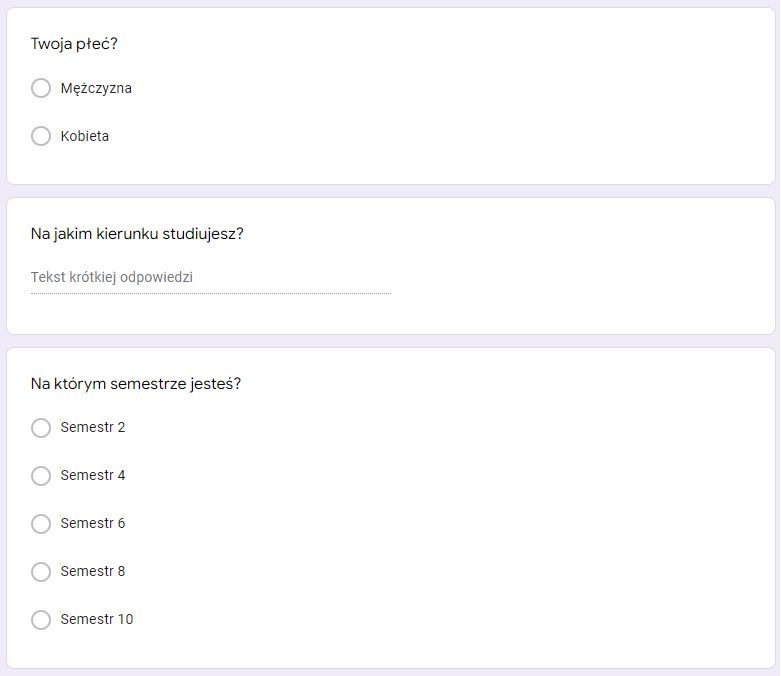
\includegraphics[width=\maxwidth]{ankieta1} 
\end{knitrout}
\newline
\textbf{Przykładowe pytania:}\newline
\begin{knitrout}
\definecolor{shadecolor}{rgb}{0.969, 0.969, 0.969}\color{fgcolor}
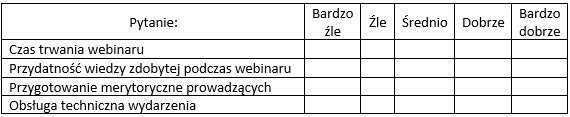
\includegraphics[width=\maxwidth]{ankieta2} 
\end{knitrout}
\newline
Taką ankietę możemy stworzyć za pomocą darmowych narzędzi dostępnych w internecie, na przykład Formularze Google.
\newline
\newline
\newline
\section*{Lista 3}
\subsection*{Zad 1}
Przeprowadzić symulacje, których celem jest porównanie prawdopodobieństwa pokrycia i długości przedziałów ufności Cloppera-Pearsona, Walda i trzeciego dowolnego typu przedziału ufności zaimplementowanego w funkcji \textit{binom.confint} pakietu \textit{binom}. Uwzględnić poziom ufności 0.95, różne rozmiary próby i różne wartości prawdopodobieństwa $p$. Wyniki zamieścić w tabelach i na rysunkach. Sformułować wnioski, które umożliwią praktykowi wybór konkretnego przedziału ufności do wyznaczenia jego realizacji dla konkretnych danych.\\

W symulacji wykorzystamy przedziały ufności Cloppera-Pearsona, Walda i Asymptotyczne.Jako trzecią metodę wybraliśmy test asymptotyczny, ponieważ znacząco różni się od dwóch pozostałych. Wykorzystuje on Centralne Twierdzenie Graniczne, więc powinien bardzo dobrze działać dla próbki o dużym rozmiarze.
Symulacje przeprowadzimy na podstawie realizacji zmiennej losowej: $X \sim \mathcal{B}(n, p)$. Wyznaczymy prawdopodobieństwa pokrycia oraz długości przedziałów ufności, a wykorzystamy do tego symulacje Monte Carlo.  \newline\newline
Poniżej znajduje się kod z symulacją:
\begin{knitrout}
\definecolor{shadecolor}{rgb}{0.969, 0.969, 0.969}\color{fgcolor}\begin{kframe}
\begin{alltt}
\hlstd{symulation} \hlkwb{<-}\hlkwa{function}\hlstd{(}\hlkwc{n} \hlstd{=} \hlnum{10}\hlstd{,} \hlkwc{dp}\hlstd{=} \hlnum{0.2}\hlstd{,} \hlkwc{MCs} \hlstd{=} \hlnum{1000}\hlstd{)\{}
  \hlstd{ps} \hlkwb{<-} \hlkwd{seq}\hlstd{(}\hlnum{0.01}\hlstd{,} \hlnum{0.99}\hlstd{, dp)}
  \hlstd{N} \hlkwb{<-} \hlkwd{length}\hlstd{(ps)}
  \hlstd{data} \hlkwb{<-} \hlkwd{matrix}\hlstd{(}\hlnum{0}\hlstd{,N,}\hlnum{6}\hlstd{)}

  \hlkwa{for} \hlstd{(k} \hlkwa{in} \hlnum{1}\hlopt{:}\hlstd{N) \{}
    \hlstd{p} \hlkwb{<-} \hlstd{ps[k]}
    \hlstd{wilson_ok} \hlkwb{<-} \hlnum{0}
    \hlstd{axact_ok}  \hlkwb{<-} \hlnum{0}
    \hlstd{asymp_ok}  \hlkwb{<-} \hlnum{0}
    \hlstd{wilson_l} \hlkwb{<-} \hlkwd{rep}\hlstd{(}\hlnum{0}\hlstd{,MCs)}
    \hlstd{axact_l}  \hlkwb{<-} \hlkwd{rep}\hlstd{(}\hlnum{0}\hlstd{,MCs)}
    \hlstd{asymp_l}  \hlkwb{<-} \hlkwd{rep}\hlstd{(}\hlnum{0}\hlstd{,MCs)}

    \hlkwa{for} \hlstd{(i} \hlkwa{in} \hlnum{1}\hlopt{:}\hlstd{MCs)\{}
      \hlstd{x} \hlkwb{<-} \hlkwd{rbinom}\hlstd{(}\hlnum{1}\hlstd{, n, p)}
      \hlstd{wilson} \hlkwb{<-} \hlkwd{binom.wilson}\hlstd{(x, n)}
      \hlstd{exact}  \hlkwb{<-} \hlkwd{binom.exact}\hlstd{(x, n)}
      \hlstd{asymp}  \hlkwb{<-} \hlkwd{binom.asymp}\hlstd{(x, n)}
      \hlstd{wilson_l[i]} \hlkwb{<-} \hlstd{wilson}\hlopt{$}\hlstd{upper} \hlopt{-} \hlstd{wilson}\hlopt{$}\hlstd{lower}
      \hlstd{axact_l[i]} \hlkwb{<-} \hlstd{exact}\hlopt{$}\hlstd{upper} \hlopt{-} \hlstd{exact}\hlopt{$}\hlstd{lower}
      \hlstd{asymp_l[i]} \hlkwb{<-} \hlstd{asymp}\hlopt{$}\hlstd{upper} \hlopt{-} \hlstd{asymp}\hlopt{$}\hlstd{lower}

      \hlkwa{if} \hlstd{(wilson[}\hlstr{"lower"}\hlstd{]}\hlopt{<}\hlstd{p} \hlopt{&&} \hlstd{p} \hlopt{<} \hlstd{wilson[}\hlstr{"upper"}\hlstd{]) \{}
        \hlstd{wilson_ok} \hlkwb{<-} \hlnum{1} \hlopt{+} \hlstd{wilson_ok}
      \hlstd{\}}
      \hlkwa{if} \hlstd{(exact[}\hlstr{"lower"}\hlstd{]}\hlopt{<}\hlstd{p} \hlopt{&&} \hlstd{p} \hlopt{<} \hlstd{exact[}\hlstr{"upper"}\hlstd{]) \{}
        \hlstd{axact_ok} \hlkwb{<-} \hlnum{1} \hlopt{+} \hlstd{axact_ok}
      \hlstd{\}}
      \hlkwa{if} \hlstd{(asymp[}\hlstr{"lower"}\hlstd{]}\hlopt{<}\hlstd{p} \hlopt{&&} \hlstd{p} \hlopt{<} \hlstd{asymp[}\hlstr{"upper"}\hlstd{]) \{}
        \hlstd{asymp_ok} \hlkwb{<-} \hlnum{1} \hlopt{+} \hlstd{asymp_ok}
      \hlstd{\}}
    \hlstd{\}}

    \hlstd{data[k,]}\hlkwb{<-} \hlkwd{c}\hlstd{( wilson_ok}\hlopt{/}\hlstd{MCs, axact_ok}\hlopt{/}\hlstd{MCs, asymp_ok}\hlopt{/}\hlstd{MCs,}
                  \hlkwd{mean}\hlstd{(wilson_l),} \hlkwd{mean}\hlstd{(axact_l),} \hlkwd{mean}\hlstd{(asymp_l))}
  \hlstd{\}}
  \hlkwd{return}\hlstd{(data)}
\hlstd{\}}
\end{alltt}
\end{kframe}
\end{knitrout}
Symulacje przeprowadzamy dla $n=10$ z krokiem równym $dp = 0.01$. Wyniki zapisujemy w pliku csv, dzięki czemu nie musimy za każdym razem czekać na wyniki.
\begin{knitrout}
\definecolor{shadecolor}{rgb}{0.969, 0.969, 0.969}\color{fgcolor}\begin{kframe}
\begin{alltt}
\hlstd{data} \hlkwb{<-} \hlkwd{symulation}\hlstd{(}\hlkwc{n} \hlstd{=} \hlnum{10}\hlstd{,} \hlkwc{dp} \hlstd{=} \hlnum{0.01}\hlstd{)}
\hlkwd{write.csv}\hlstd{(df_l,} \hlstr{"data_n_10.csv"}\hlstd{)}
\end{alltt}
\end{kframe}
\end{knitrout}

Stwórzmy teraz ramki danych prawdopodobieństw pokrycia:
\begin{knitrout}
\definecolor{shadecolor}{rgb}{0.969, 0.969, 0.969}\color{fgcolor}\begin{kframe}
\begin{alltt}
\hlstd{data} \hlkwb{<-} \hlkwd{read.csv}\hlstd{(}\hlstr{"data_n_10.csv"}\hlstd{)}
\hlstd{ps} \hlkwb{<-} \hlkwd{seq}\hlstd{(}\hlnum{0.01}\hlstd{,} \hlnum{0.99}\hlstd{,} \hlnum{0.01}\hlstd{)}
\hlstd{df1} \hlkwb{<-} \hlkwd{data.frame}\hlstd{(}\hlkwc{wilsonp} \hlstd{= data[,}\hlnum{1}\hlstd{],} \hlkwc{axact} \hlstd{= data[,}\hlnum{2}\hlstd{],}
                    \hlkwc{asymp} \hlstd{= data[,}\hlnum{3}\hlstd{],} \hlkwc{p} \hlstd{= ps)}
\hlkwd{head}\hlstd{(df1)}
\end{alltt}
\begin{verbatim}
##   wilsonp axact asymp    p
## 1   0.895 0.997 0.105 0.01
## 2   0.980 0.980 0.194 0.02
## 3   0.967 0.997 0.259 0.03
## 4   0.952 0.996 0.313 0.04
## 5   0.922 0.991 0.369 0.05
## 6   0.990 0.990 0.498 0.06
\end{verbatim}
\end{kframe}
\end{knitrout}
Stwórzmy teraz ramki danych średniej długości przedziałów:
\begin{knitrout}
\definecolor{shadecolor}{rgb}{0.969, 0.969, 0.969}\color{fgcolor}\begin{kframe}
\begin{alltt}
\hlstd{df2} \hlkwb{<-} \hlkwd{data.frame}\hlstd{(}\hlkwc{wilsonp} \hlstd{= data[,}\hlnum{4}\hlstd{],} \hlkwc{axact} \hlstd{= data[,}\hlnum{5}\hlstd{],}
                    \hlkwc{asymp} \hlstd{= data[,}\hlnum{6}\hlstd{],} \hlkwc{p} \hlstd{= ps)}
\hlkwd{head}\hlstd{(df2)}
\end{alltt}
\begin{verbatim}
##     wilsonp     axact      asymp    p
## 1 0.2891513 0.3228313 0.03941896 0.01
## 2 0.3000085 0.3363140 0.07469554 0.02
## 3 0.3080306 0.3462822 0.10062344 0.03
## 4 0.3152131 0.3552272 0.12345860 0.04
## 5 0.3233879 0.3654924 0.14795246 0.05
## 6 0.3416031 0.3883001 0.20384545 0.06
\end{verbatim}
\end{kframe}
\end{knitrout}
Sprawdzamy również wykresy:
\begin{knitrout}
\definecolor{shadecolor}{rgb}{0.969, 0.969, 0.969}\color{fgcolor}\begin{kframe}
\begin{alltt}
\hlstd{df_p} \hlkwb{<-} \hlkwd{melt}\hlstd{(df1,}\hlkwc{id.vars}\hlstd{=}\hlstr{"p"}\hlstd{)}
\hlkwd{ggplot}\hlstd{(df_p,}\hlkwd{aes}\hlstd{(p, value,}\hlkwc{col}\hlstd{=variable))}\hlopt{+}
  \hlkwd{geom_point}\hlstd{()}\hlopt{+} \hlkwd{geom_line}\hlstd{()}
\end{alltt}
\end{kframe}\begin{figure}[H]
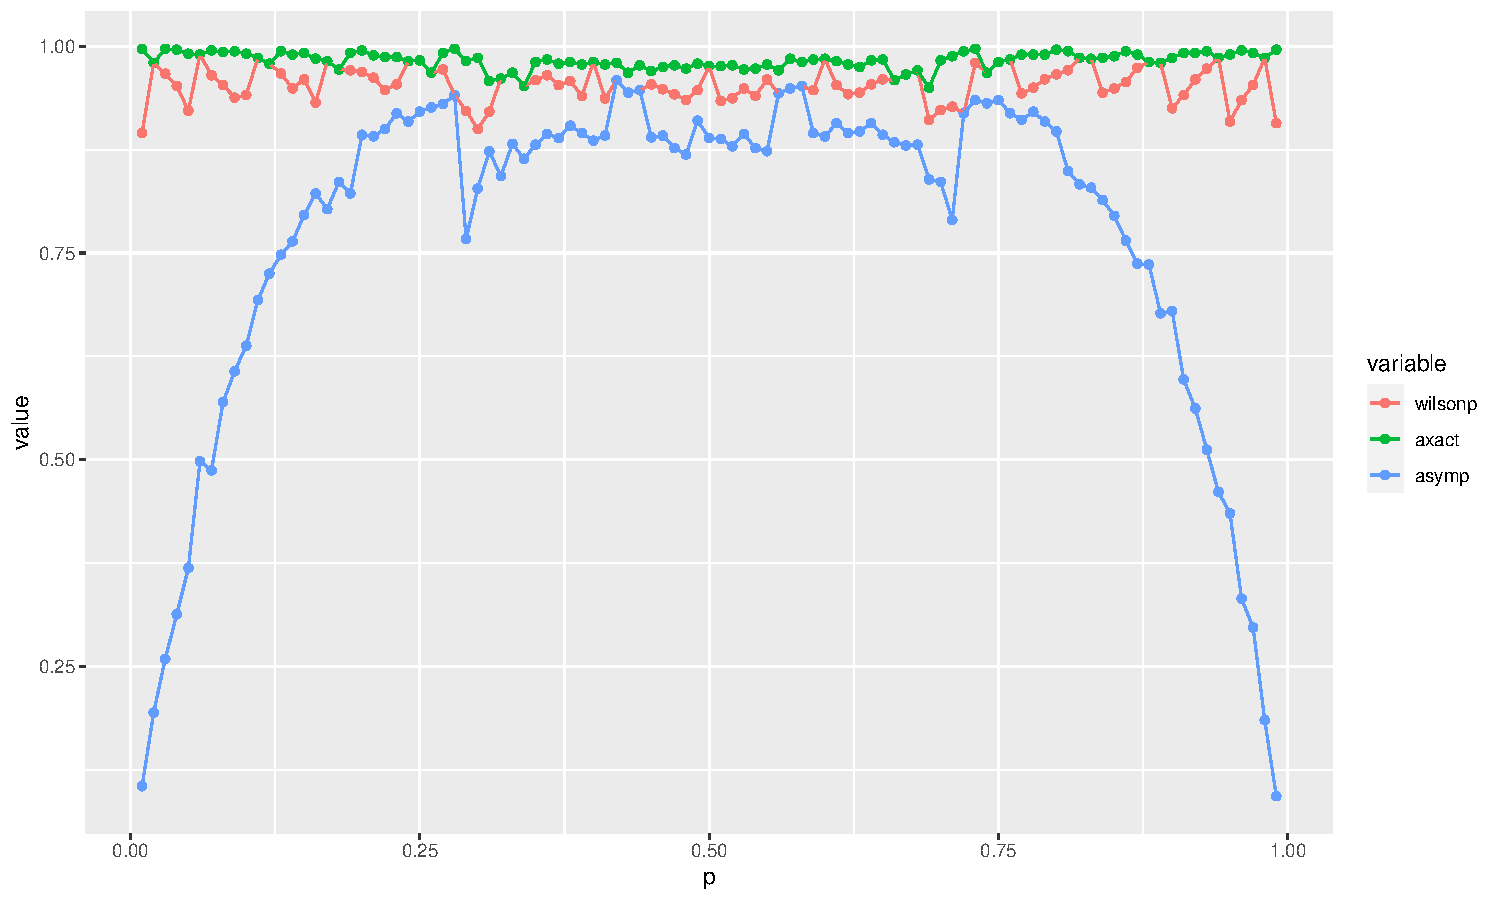
\includegraphics[width=\maxwidth]{figure/fig_6-1} \caption{\label{fig:6}Wykres prawdopodobieństwa pokrycia dla poszczególnych metod i n równego 10.}\label{fig:fig_6}
\end{figure}

\end{knitrout}
\begin{knitrout}
\definecolor{shadecolor}{rgb}{0.969, 0.969, 0.969}\color{fgcolor}\begin{kframe}
\begin{alltt}
\hlstd{df_l} \hlkwb{<-} \hlkwd{melt}\hlstd{(df2,}\hlkwc{id.vars}\hlstd{=}\hlstr{"p"}\hlstd{)}
\hlkwd{ggplot}\hlstd{(df_l,}\hlkwd{aes}\hlstd{(p, value,}\hlkwc{col}\hlstd{=variable))}\hlopt{+}
  \hlkwd{geom_point}\hlstd{()}\hlopt{+} \hlkwd{geom_line}\hlstd{()}
\end{alltt}
\end{kframe}\begin{figure}[H]
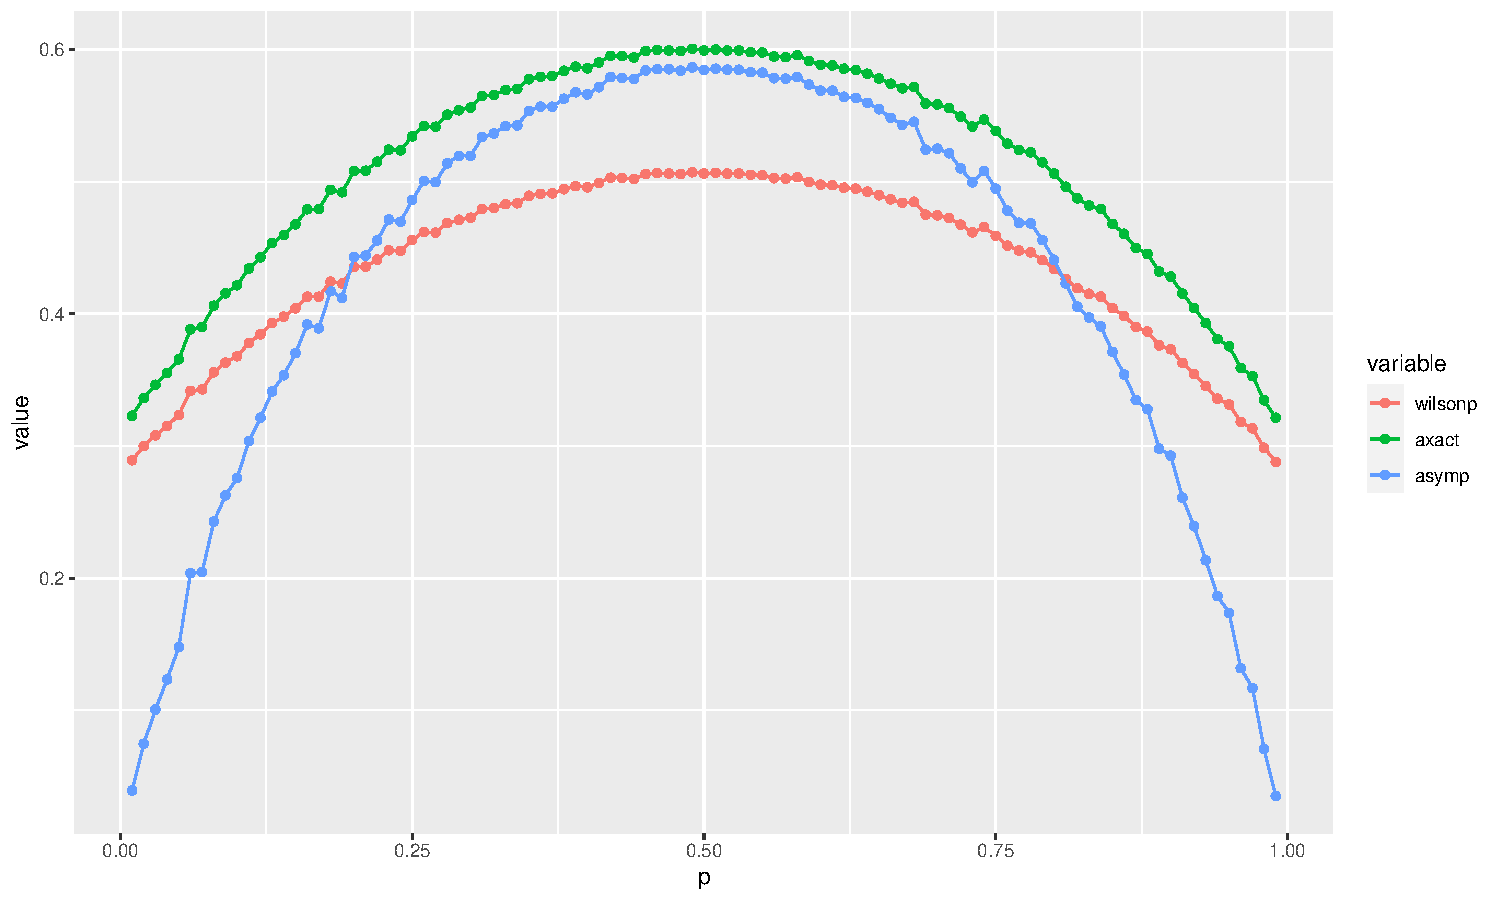
\includegraphics[width=\maxwidth]{figure/fig_7-1} \caption{\label{fig:7}Wykres średniej długości przedziałów dla poszczególnych metod i n równego 10.}\label{fig:fig_7}
\end{figure}

\end{knitrout}
Zobaczmy również jak wygladają powyższe wykresy, ale tym razem dla n równego 100:

\begin{knitrout}
\definecolor{shadecolor}{rgb}{0.969, 0.969, 0.969}\color{fgcolor}\begin{figure}[H]
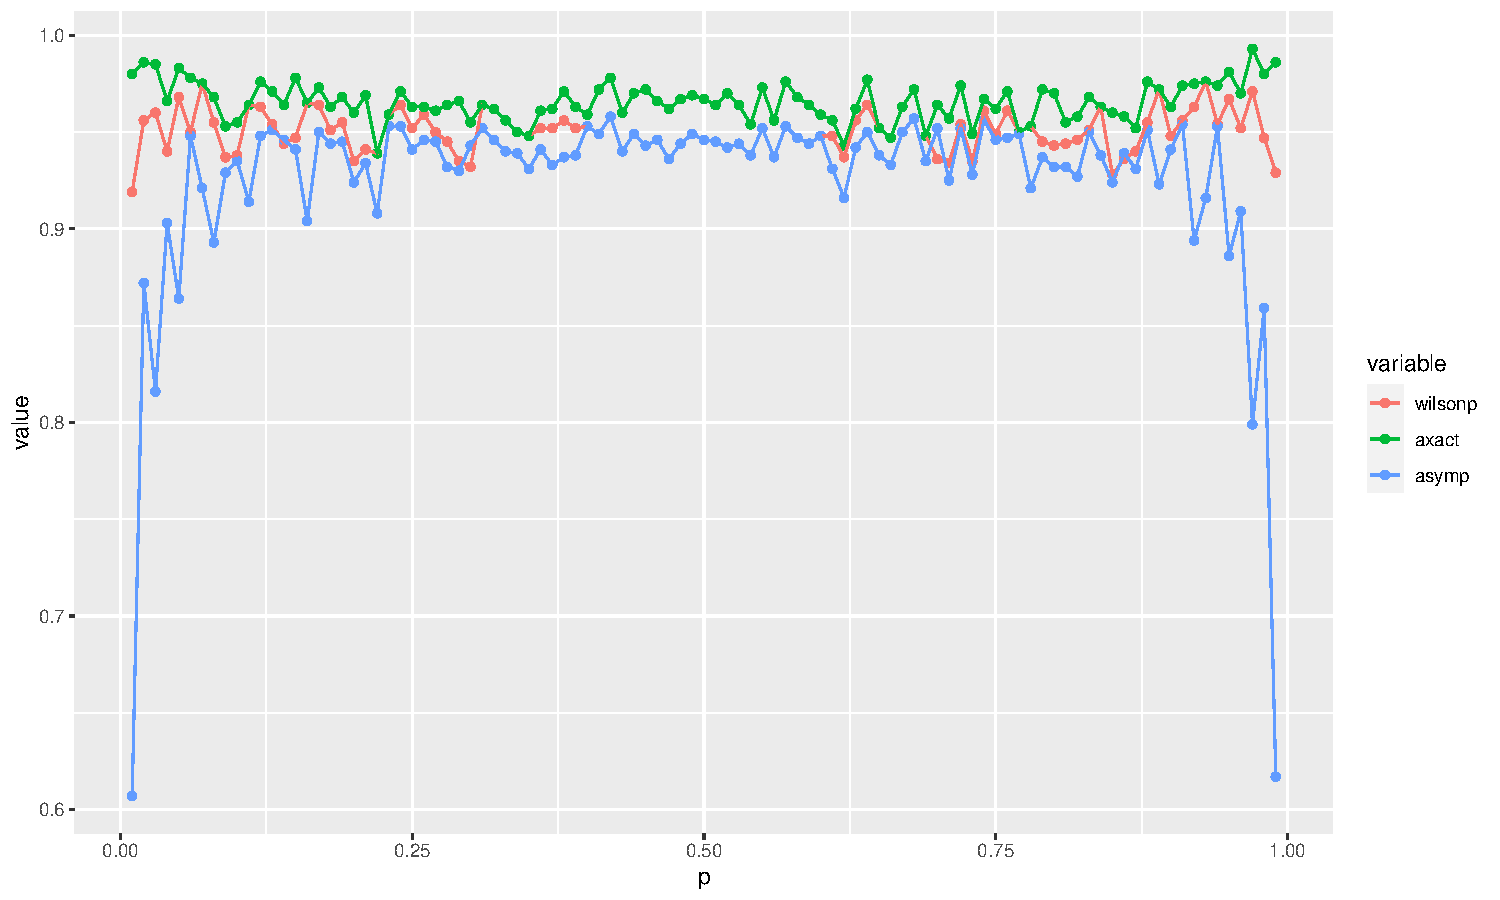
\includegraphics[width=\maxwidth]{figure/fig_8-1} \caption{\label{fig:8}Wykres prawdopodobieństwa pokrycia dla poszczególnych metod i n równego 100.}\label{fig:fig_8}
\end{figure}

\end{knitrout}
\begin{knitrout}
\definecolor{shadecolor}{rgb}{0.969, 0.969, 0.969}\color{fgcolor}\begin{figure}[H]
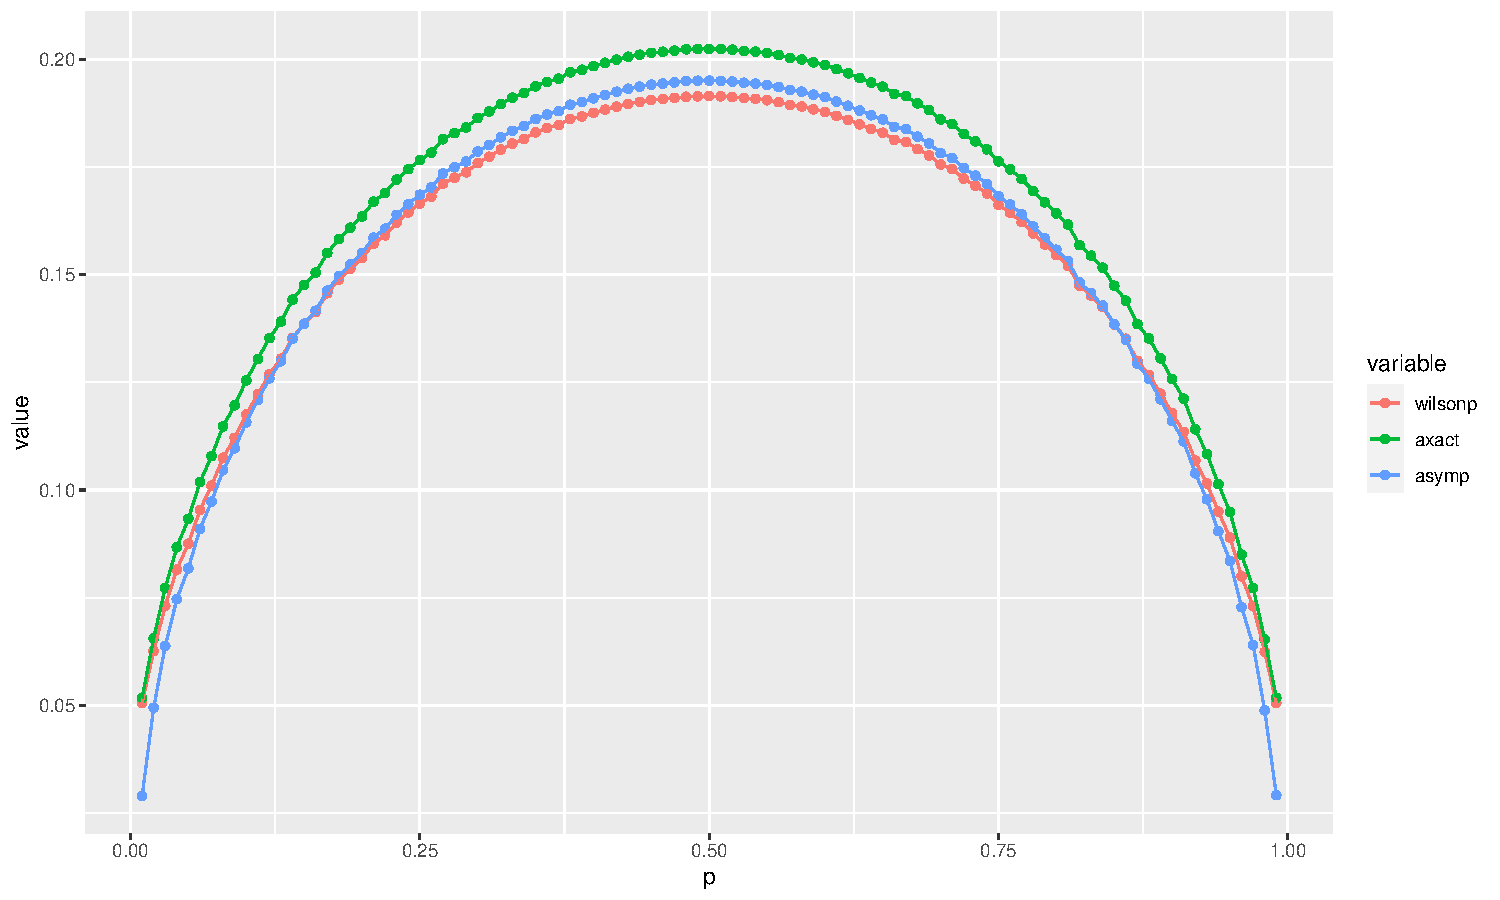
\includegraphics[width=\maxwidth]{figure/fig_9-1} \caption{\label{fig:9}Wykres średniej długości przedziałów dla poszczególnych metod i n równego 100.}\label{fig:fig_9}
\end{figure}

\end{knitrout}
\subsection*{Porównanie Rysunku \ref{fig:6} z Rysunkiem \ref{fig:8}:} 
% ######################################## może do usuniecia
\begin{knitrout}
\definecolor{shadecolor}{rgb}{0.969, 0.969, 0.969}\color{fgcolor}\begin{figure}[H]
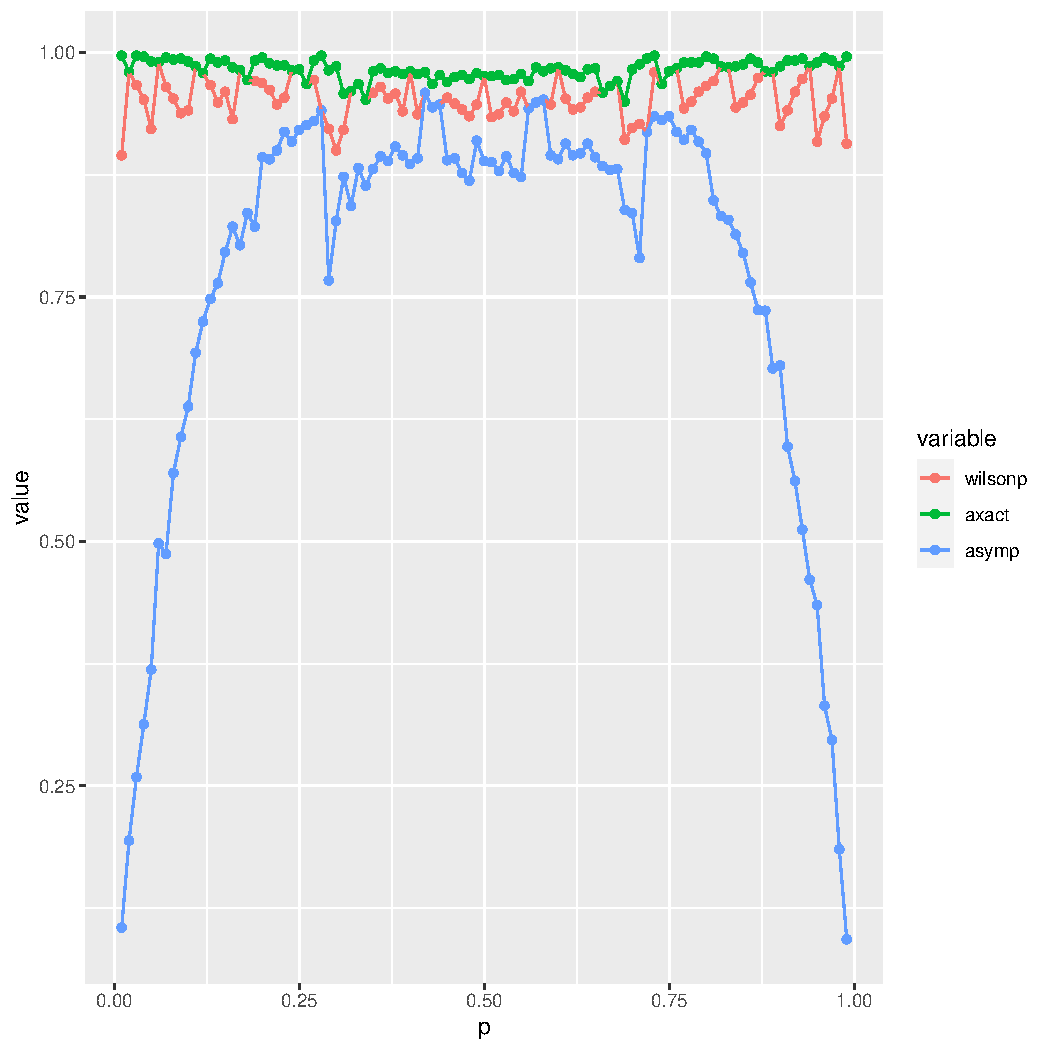
\includegraphics[width=0.5\linewidth]{figure/fig_10-1} 
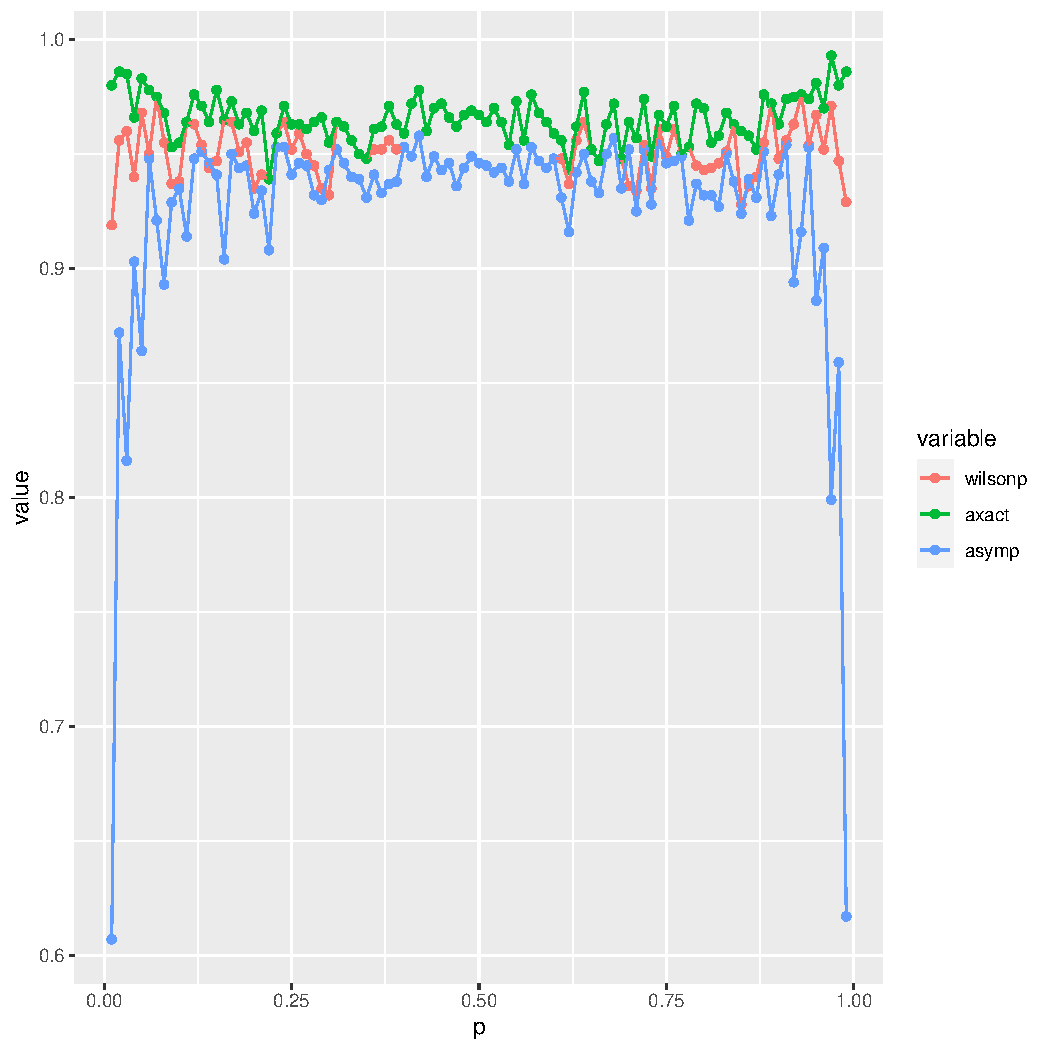
\includegraphics[width=0.5\linewidth]{figure/fig_10-2} \caption{\label{fig:10}Wykresy prawdopodobieństwa pokrycia dla poszczególnych metod i n równego odpowiednio 10 i 100.}\label{fig:fig_10}
\end{figure}

\end{knitrout}
\newpage
\subsection*{Porównanie Rysunku \ref{fig:7} z Rysunkiem \ref{fig:9}:}
\begin{knitrout}
\definecolor{shadecolor}{rgb}{0.969, 0.969, 0.969}\color{fgcolor}\begin{figure}[H]
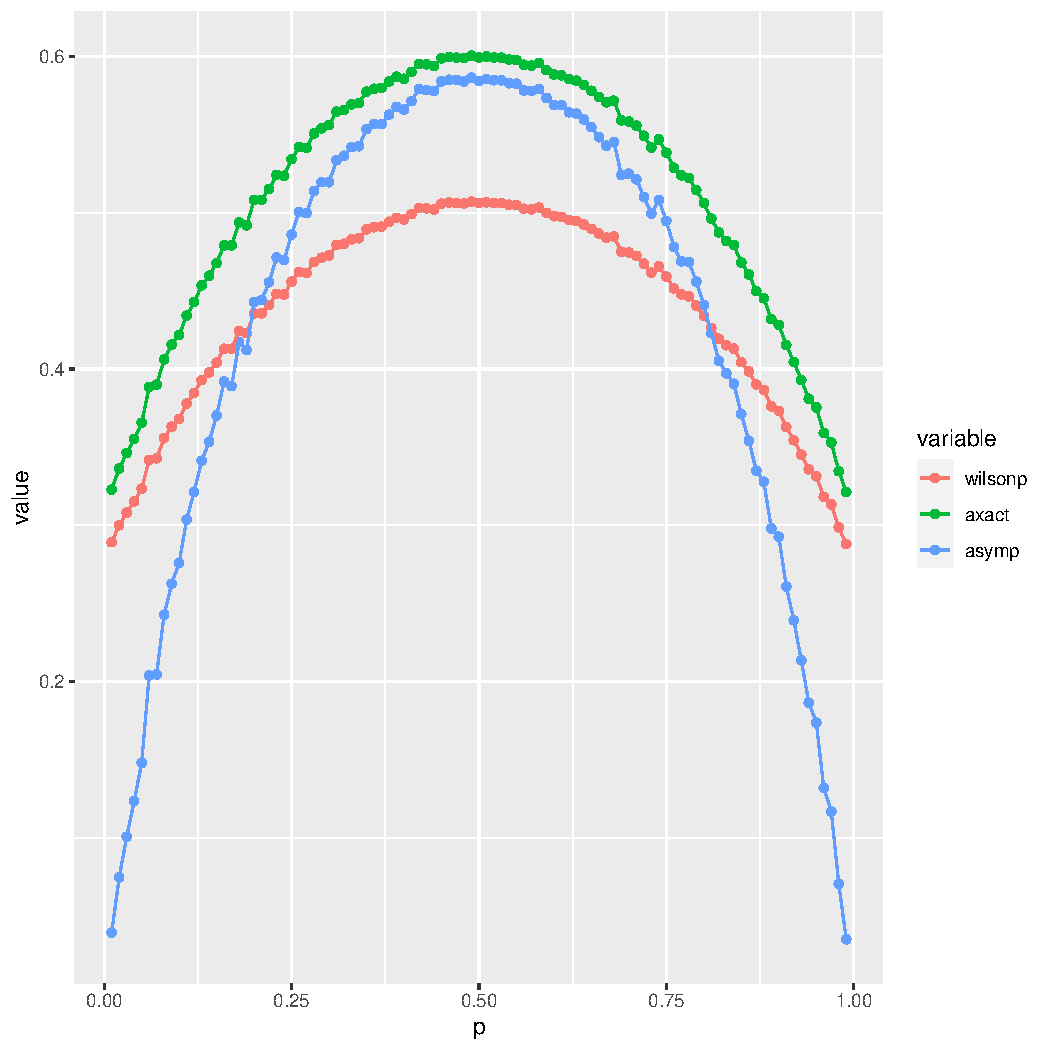
\includegraphics[width=0.5\linewidth]{figure/fig_11-1} 
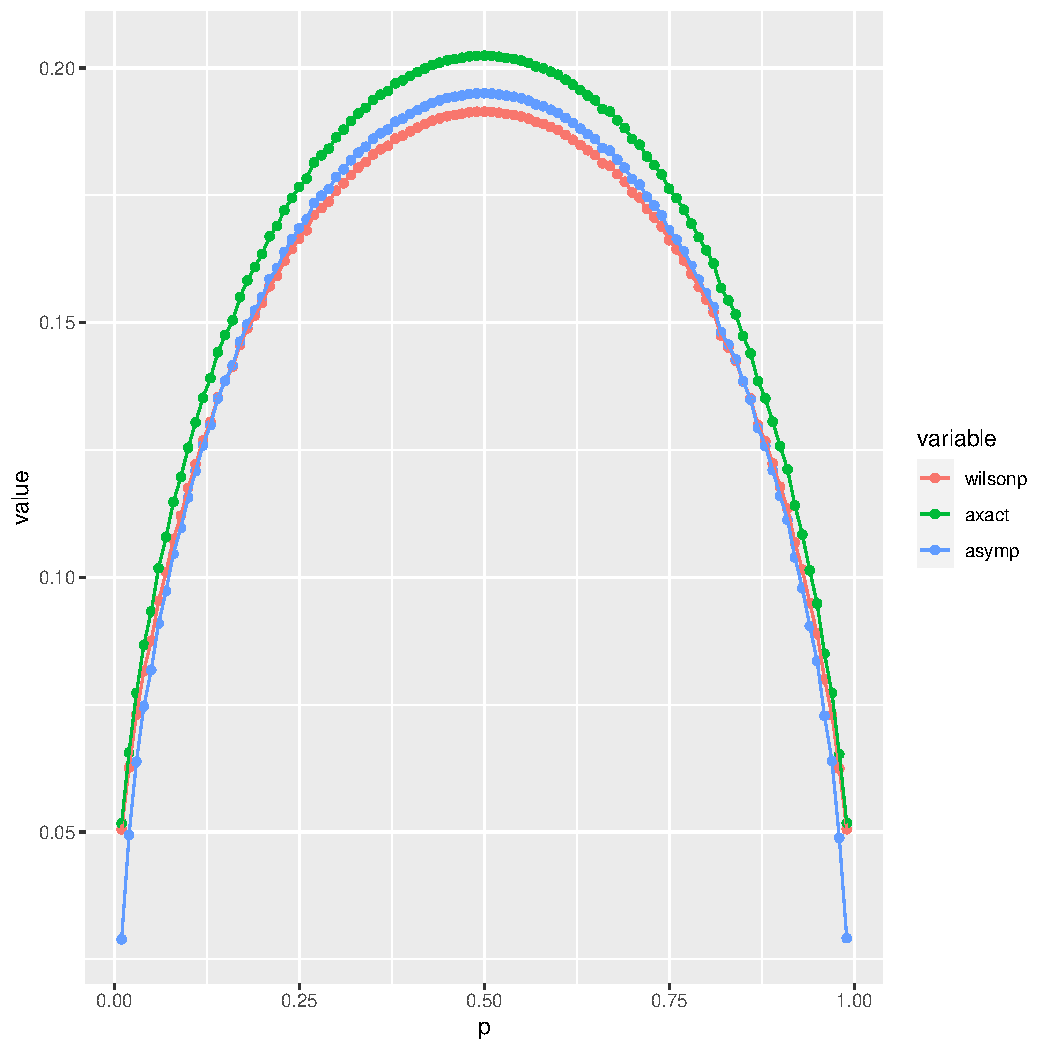
\includegraphics[width=0.5\linewidth]{figure/fig_11-2} \caption{\label{fig:11}Wykresy średniej długości przedziałów dla poszczególnych metod i n równego 10 i 100.}\label{fig:fig_11}
\end{figure}

\end{knitrout}
% #######################################
\textbf{Wnioski:}\newline
Jak możemy zobaczyć z powyższych wykresów, przedziały Cloppera-Pearsona mają największe prawdopodobieństwo pokrycia oraz największą średnią długość dla każdego $p$, świadczy to, że metoda Cloppera-Pearsona będzie najlepszym wyborem spośród testowanych metod. Zdecydowanie najgorszym okazał się test asymptotyczny, okazało się, że ta metoda wymaga jeszcze większych rozmiarów próbki.

\newpage
\subsection*{Zad 2}
Załóżmy, że 200 losowo wybranych klientów (w różnym wieku) kilku (losowo wybranych) aptek zapytano, jaki lek przeciwbólowy zwykle stosują. Zebrane dane zawarte są w tablicy 1. Na podstawie tych danych, wyznaczyć realizacje przedziałów ufności, na poziomie ufności 0.95. \newline
\newline
Do wyboru najlepszych przedziałów ufności stosujemy funkcję $binom.confint$. Funkcja ta zwraca tabelkę z porównaniem 11 metod. Przedziały będziemy porównywać na podstawie ich długości, im węższy tym metoda jest lepsza. Długość takiego przedziału będzie opisana w tabelce w kolumnie $ls$.\newline
\subsubsection*{a) Prawdopodobieństwo stosowania leku ibuprofen (bez względu na grupę wiekową)}
\begin{knitrout}\small
\definecolor{shadecolor}{rgb}{0.969, 0.969, 0.969}\color{fgcolor}\begin{kframe}
\begin{alltt}
\hlstd{conf} \hlkwb{<-} \hlkwd{binom.confint}\hlstd{(}\hlnum{50}\hlstd{,}\hlnum{200}\hlstd{)}
\hlstd{ls} \hlkwb{<-} \hlstd{conf}\hlopt{$}\hlstr{"upper"}\hlopt{-} \hlstd{conf}\hlopt{$}\hlstr{"lower"}
\hlkwd{cbind}\hlstd{(conf,ls)}
\end{alltt}
\begin{verbatim}
##           method  x   n      mean     lower     upper        ls
## 1  agresti-coull 50 200 0.2500000 0.1948993 0.3145233 0.1196240
## 2     asymptotic 50 200 0.2500000 0.1899886 0.3100114 0.1200228
## 3          bayes 50 200 0.2512438 0.1923105 0.3115641 0.1192536
## 4        cloglog 50 200 0.2500000 0.1923621 0.3116476 0.1192856
## 5          exact 50 200 0.2500000 0.1916072 0.3159628 0.1243557
## 6          logit 50 200 0.2500000 0.1948697 0.3146322 0.1197625
## 7         probit 50 200 0.2500000 0.1939760 0.3136105 0.1196346
## 8        profile 50 200 0.2500000 0.1934176 0.3129498 0.1195322
## 9            lrt 50 200 0.2500000 0.1934316 0.3129489 0.1195173
## 10     prop.test 50 200 0.2500000 0.1928239 0.3169864 0.1241625
## 11        wilson 50 200 0.2500000 0.1950817 0.3143410 0.1192593
\end{verbatim}
\end{kframe}
\end{knitrout}
Dla tych danych najlepsza okazała się $metoda Bayes'a$.
\begin{knitrout}\small
\definecolor{shadecolor}{rgb}{0.969, 0.969, 0.969}\color{fgcolor}\begin{kframe}
\begin{alltt}
\hlkwd{cbind}\hlstd{(conf,ls)[ls} \hlopt{==} \hlkwd{min}\hlstd{(ls),]}
\end{alltt}
\begin{verbatim}
##   method  x   n      mean     lower     upper        ls
## 3  bayes 50 200 0.2512438 0.1923105 0.3115641 0.1192536
\end{verbatim}
\end{kframe}
\end{knitrout}

\newpage
\subsubsection*{b) Prawdopodobieństwo stosowania leku ibuprofen przez klienta w wieku do 35
lat}
\begin{knitrout}\small
\definecolor{shadecolor}{rgb}{0.969, 0.969, 0.969}\color{fgcolor}\begin{kframe}
\begin{alltt}
\hlstd{conf} \hlkwb{<-} \hlkwd{binom.confint}\hlstd{(}\hlnum{0}\hlstd{,}\hlnum{90}\hlstd{)}
\hlstd{ls} \hlkwb{<-} \hlstd{conf}\hlopt{$}\hlstr{"upper"}\hlopt{-} \hlstd{conf}\hlopt{$}\hlstr{"lower"}
\hlkwd{cbind}\hlstd{(conf,ls)}
\end{alltt}
\begin{verbatim}
##           method x  n        mean        lower      upper         ls
## 1  agresti-coull 0 90 0.000000000 -0.008180285 0.04911591 0.05729620
## 2     asymptotic 0 90 0.000000000  0.000000000 0.00000000 0.00000000
## 3          bayes 0 90 0.005494505  0.000000000 0.02105727 0.02105727
## 4        cloglog 0 90 0.000000000  0.000000000 0.04015892 0.04015892
## 5          exact 0 90 0.000000000  0.000000000 0.04015892 0.04015892
## 6          logit 0 90 0.000000000  0.000000000 0.04015892 0.04015892
## 7         probit 0 90 0.000000000  0.000000000 0.04015892 0.04015892
## 8        profile 0 90 0.000000000  0.000000000 0.03652208 0.03652208
## 9            lrt 0 90 0.000000000  0.000000000 0.02111561 0.02111561
## 10     prop.test 0 90 0.000000000  0.000000000 0.05101162 0.05101162
## 11        wilson 0 90 0.000000000  0.000000000 0.04093563 0.04093563
\end{verbatim}
\end{kframe}
\end{knitrout}

Najlepszy w tym przypadku okazał się test asymptotyczny.
\begin{knitrout}\small
\definecolor{shadecolor}{rgb}{0.969, 0.969, 0.969}\color{fgcolor}\begin{kframe}
\begin{alltt}
\hlkwd{cbind}\hlstd{(conf,ls)[ls} \hlopt{==} \hlkwd{min}\hlstd{(ls),]}
\end{alltt}
\begin{verbatim}
##       method x  n mean lower upper ls
## 2 asymptotic 0 90    0     0     0  0
\end{verbatim}
\end{kframe}
\end{knitrout}


\subsubsection*{c) Prawdopodobieństwo stosowania leku apap (bez względu na grupę wiekową)}
\begin{knitrout}\small
\definecolor{shadecolor}{rgb}{0.969, 0.969, 0.969}\color{fgcolor}\begin{kframe}
\begin{alltt}
\hlstd{conf} \hlkwb{<-} \hlkwd{binom.confint}\hlstd{(}\hlnum{44}\hlstd{,}\hlnum{200}\hlstd{)}
\hlstd{ls} \hlkwb{<-} \hlstd{conf}\hlopt{$}\hlstr{"upper"}\hlopt{-} \hlstd{conf}\hlopt{$}\hlstr{"lower"}
\hlkwd{cbind}\hlstd{(conf,ls)}
\end{alltt}
\begin{verbatim}
##           method  x   n     mean     lower     upper        ls
## 1  agresti-coull 44 200 0.220000 0.1679267 0.2826267 0.1147000
## 2     asymptotic 44 200 0.220000 0.1625894 0.2774106 0.1148211
## 3          bayes 44 200 0.221393 0.1651366 0.2792052 0.1140686
## 4        cloglog 44 200 0.220000 0.1654772 0.2795930 0.1141158
## 5          exact 44 200 0.220000 0.1646361 0.2838612 0.1192252
## 6          logit 44 200 0.220000 0.1679499 0.2827004 0.1147504
## 7         probit 44 200 0.220000 0.1670005 0.2815308 0.1145304
## 8        profile 44 200 0.220000 0.1663740 0.2807561 0.1143821
## 9            lrt 44 200 0.220000 0.1663832 0.2807552 0.1143720
## 10     prop.test 44 200 0.220000 0.1659406 0.2850661 0.1191255
## 11        wilson 44 200 0.220000 0.1681654 0.2823880 0.1142226
\end{verbatim}
\end{kframe}
\end{knitrout}
Po raz drugi test $Bayes'a$ okazuję się najlepszy.
\begin{knitrout}\small
\definecolor{shadecolor}{rgb}{0.969, 0.969, 0.969}\color{fgcolor}\begin{kframe}
\begin{alltt}
\hlkwd{cbind}\hlstd{(conf,ls)[ls} \hlopt{==} \hlkwd{min}\hlstd{(ls),]}
\end{alltt}
\begin{verbatim}
##   method  x   n     mean     lower     upper        ls
## 3  bayes 44 200 0.221393 0.1651366 0.2792052 0.1140686
\end{verbatim}
\end{kframe}
\end{knitrout}


\subsubsection*{d) Prawdopodobieństwo stosowania leku apap przez klienta w wieku do 35 lat}
\begin{knitrout}\small
\definecolor{shadecolor}{rgb}{0.969, 0.969, 0.969}\color{fgcolor}\begin{kframe}
\begin{alltt}
\hlstd{conf} \hlkwb{<-} \hlkwd{binom.confint}\hlstd{(}\hlnum{22}\hlstd{,}\hlnum{90}\hlstd{)}
\hlstd{ls} \hlkwb{<-} \hlstd{conf}\hlopt{$}\hlstr{"upper"}\hlopt{-} \hlstd{conf}\hlopt{$}\hlstr{"lower"}
\hlkwd{cbind}\hlstd{(conf,ls)}
\end{alltt}
\begin{verbatim}
##           method  x  n      mean     lower     upper        ls
## 1  agresti-coull 22 90 0.2444444 0.1667306 0.3430809 0.1763503
## 2     asymptotic 22 90 0.2444444 0.1556573 0.3332316 0.1775743
## 3          bayes 22 90 0.2472527 0.1612799 0.3363365 0.1750565
## 4        cloglog 22 90 0.2444444 0.1615228 0.3366897 0.1751669
## 5          exact 22 90 0.2444444 0.1599693 0.3463767 0.1864074
## 6          logit 22 90 0.2444444 0.1667000 0.3435007 0.1768006
## 7         probit 22 90 0.2444444 0.1648158 0.3411605 0.1763447
## 8        profile 22 90 0.2444444 0.1636309 0.3396167 0.1759858
## 9            lrt 22 90 0.2444444 0.1636231 0.3396152 0.1759921
## 10     prop.test 22 90 0.2444444 0.1626454 0.3484391 0.1857937
## 11        wilson 22 90 0.2444444 0.1673278 0.3424837 0.1751559
\end{verbatim}
\end{kframe}
\end{knitrout}
W podpunkcie $d) $ najlepszym testem jest po raz trzeci test $Bayes'a$.
\begin{knitrout}\small
\definecolor{shadecolor}{rgb}{0.969, 0.969, 0.969}\color{fgcolor}\begin{kframe}
\begin{alltt}
\hlkwd{cbind}\hlstd{(conf,ls)[ls} \hlopt{==} \hlkwd{min}\hlstd{(ls),]}
\end{alltt}
\begin{verbatim}
##   method  x  n      mean     lower     upper        ls
## 3  bayes 22 90 0.2472527 0.1612799 0.3363365 0.1750565
\end{verbatim}
\end{kframe}
\end{knitrout}
\textbf{Wnioski:} \newline
Zauważamy, że im mamy większą liczbę sukcesów tym metody zwracają bardziej zbliżone wyniki. Największą rozbieżność mamy przy testowaniu dla liczby sukcesów równej 0, wtedy niektóre przedziały mają nawet długość 0, a inne około 0.02. Test $Bayes'a$ okazał się najlepszy w 3 podpunktach, więc możemy uznać, że jest to najlepsza metoda, którą możemy wykorzystać konstruując przedziały ufności dla tych danych.
\end{document}
